% !TeX root = ../main.tex
% Add the above to each chapter to make compiling the PDF easier in some editors.

\chapter{Evaluation}\label{chapter:evaluation}
Our original goal was to bring a first prototype fuzzer to the Algorand ecosystem of tools and for this reason we designed and implemented AlgoFuzz.
In this chapter, we will evaluate AlgoFuzz to see if it fulfills its purpose as a fuzzer for Algorand smart contracts.
The most straightforward way to find out if a fuzzer works is to see if it is able to find bugs, known and unknown.
Looking at other smart contract fuzzers, such as ContractFuzzer or Harvey, we can see that the most common approach is to run the fuzzer on real-world contracts.
After which, they would see if their fuzzer reported any bugs during the process.
In our case, since we are dealing with a property-based fuzzer and we do not have a list of predefined bug oracles, we would need to know the contracts in detail to be able to write properties that would find bugs.
Echidna, the property-based fuzzer for Ethereum, was also faced with the same problem during their evaluation.
Instead of finding bugs, they decided to see if their fuzzer was able to reach certain assertion failures which were randomly added to the contracts.

With these considerations in mind we came up with two different questions that we wanted to answer for our evaluation:
\begin{enumerate}
    \item[\textbf{RQ.1}] How effective is AlgoFuzz in terms of covering new code?

        Code coverage has been shown to correlate with the number of bugs found \cite{kochhar_code_2015}.

    \item[\textbf{RQ.2}] How effectively can AlgoFuzz discover the state space of the smart contract?

        Since the property tests are defined on the state of the contract, the more state the fuzzer discovers the more likely it is to invalidate a property.
\end{enumerate}

\section{Setup}

\subsection*{Chosen Contracts}
For our evaluation, it was difficult to find real-world Algorand smart contracts which adhered to the limitations of our fuzzer namely using the official \ac{ABI}, not using any box state and not interacting with \acp{ASA}.
For this reason we decided to write our own contracts in PyTeal based on already existing Solidity smart contracts which where used in previous works.
This way we can leverage existing contracts, while still adhering to our limitations.
The first set of contracts we chose were the twelve contracts used in the Echidna evaluation \cite{grieco_echidna_2020}, namely a subset of the VeriSmart-benchmarks \cite{noauthor_kuplverismart-benchmarks_nodate}.
For our second set of contracts we chose two contract of a larger size than the ones selected before.
The first one being the Tether stablecoin contract, presented in our case study in \ref{section:case-study}.
The second one is a generic token exchange contract, where the user can buy and sell tokens for Algos given an exchange rate, as this is a common use case for smart contracts.

\subsection*{Evaluation Protocol}
The metrics we gathered for our experiments were the ones mentioned in section \ref{section:metrics}.
We ran each configuration of the fuzzer as we did in the case study, so six configurations in total (two different fuzzing strategies and three different fuzzing drivers).
For the 12 small contracts we did 10 runs per configuration with a fuzzing time of 10 minutes each.
As these contracts are small the fuzzer should be able to reach a saturation point in this time.
In total the fuzzer ran for these contracts for 120 hours.
The two larger contracts also ran for 10 times per configuration but with a fuzzing time of 30 minutes each, as these contracts will take longer to reach a saturation point.
For the larger contracts the fuzzer ran in total for 60 hours.
All in all the experiment ran for 180 hours. After each call to the target contract we recorded the metrics in a \acs{CSV} file. The results that we show are the average of the 10 runs for each configuration.

The experiments were run on a virtual machine hosted on the LRZ Compute Cloud \cite{noauthor_lrz_nodate}.
The compute node uses Intel(R) Xeon(R) Gold 6148 CPUs at 2.40GHz.
The virtual machine had 2 CPU cores, 9 GB of RAM and 30 GB of disk space.
The operating system was Ubuntu 20.04 LTS.
AlgoFuzz used the Python 3.10.12 interpreter, the Algorand node was version 3.15.1, and the Docker version was 24.0.6.

\section{Results} \label{section:results}
In this section we will present the quantitative results of our evaluation.
We also elaborate on how the data was selected and transformed to be able to present it in a meaningful way.

From the data we collected we excluded some runs which were uncharacteristically slow, assuming that they were statistical outliers caused by the virtual machine.
The runs we excluded were the ones where the number of calls was much lower than the average for the same configuration.
These were the first 3 runs on AlgoTether contract with the Total Fuzzer and the Coverage driver.

We wanted to aggregate the data of each configuration per call.
One issue with this approach is that due to the random nature of the fuzzer, the number of calls per run was almost never the same.
For all runs in a configuration, we calculated the average, median, minimum and maximum of each metric per call.
For the averages we only considered the available data points, so if a run had no calls beyond a certain point we did not consider it for the average.
This does not affect our values since most runs achieve a similar number of calls and by the end they have all reached a saturation point.
This was only done for the graphs where we are showing the values per call.
For the final values we took the run with the least number of calls and used that index to get the final values for all runs.
In some graphs we will only be presenting the values of the larger contracts, since the smaller ones reach a saturation point very quickly and they do not change significantly after that.
Aside from that we calculated the values for the last call of each run to see what the final state of the fuzzer was.


\begin{figure}[!hbp]
    \centering
    \subfloat[AlgoTether][AlgoTether]{
        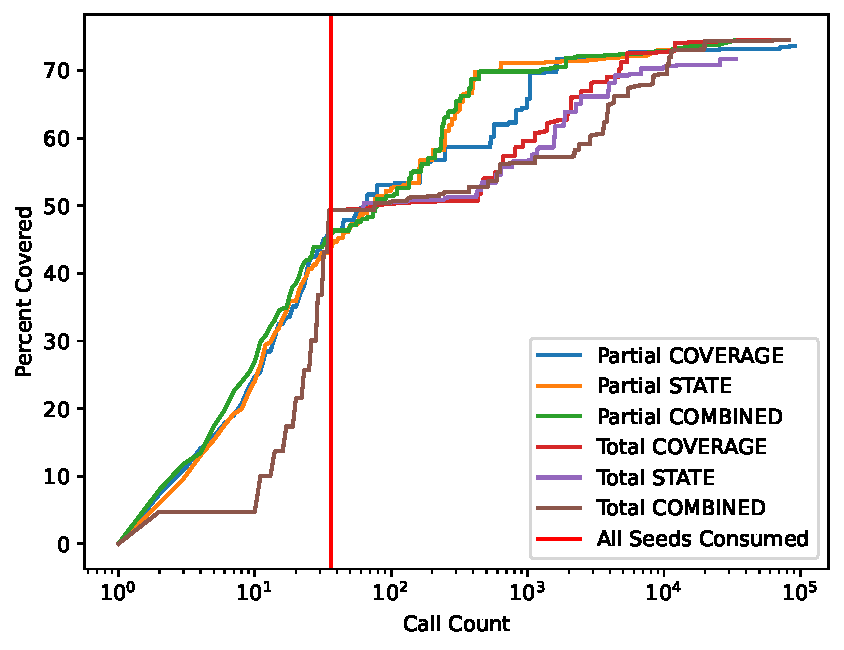
\includegraphics[width=0.48\textwidth]{charts/AlgoTether_ percent_covered_seed.pdf}
        \label{fig:AlgoTether_cov}
    }
    \hfill
    \subfloat[ExchangeToken][ExchangeToken]{
        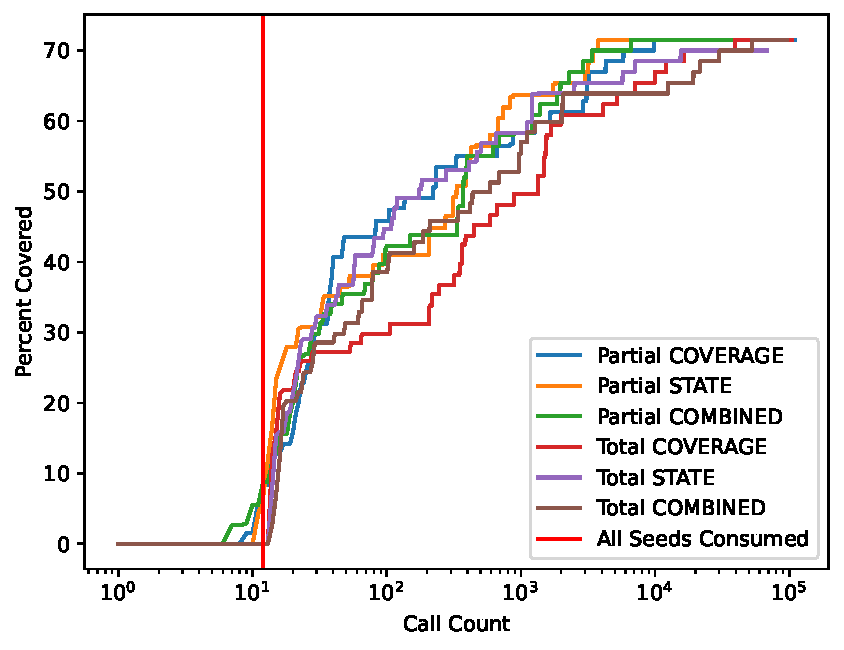
\includegraphics[width=0.48\textwidth]{charts/ExchangeToken_ percent_covered_seed.pdf}
        \label{fig:ExchangeToken_cov}
    }
    \caption{Average coverage of AlgoTether and ExchangeToken for all configurations.}
    \label{fig:percent_coverage}
\end{figure}

\subsection*{Code Coverage} \label{section:results-code-coverage}
To answer \textbf{RQ.1} we will look at percentage of code coverage over the number of calls to the target contract.
Other metrics such as lines covered or the number of unique paths covered were also considered but were discarded since they did not provide any additional information.
The percentage of code coverage is a normalized metric making it is easier to compare the results of different contracts.

In Figure \ref{fig:percent_coverage} we can see the percentage of code coverage over the number of calls for the two larger contracts.
The x axis which represents the number of calls is shown in logarithmic scale.
This is because coverage increases very quickly in the beginning and then it slows down.
We have also added a vertical line at the point where all the seed values have been consumed and after which the fuzzer is only using generated values.
All the different configurations are shown in the same graph to be able to compare them.
We can observe that the Total Fuzzer, in both cases regardless of the driver, lags behind the Partial Fuzzer.

\begin{table}[hbp]
    \centering
    \csvautotabular{data/covs-noseed-acc.csv}
    \caption{Final code coverage for each contract subtracting seed coverage.}\label{table:covs-noseed-acc}
\end{table}

Another interesting observation is that the fuzzer behaves very differently for the two contracts in the early stages.
For the AlgoTether contract, the fuzzer immediately covers new code on almost every call while consuming the seeds.
On the other hand, for the ExchangeToken contract, most of the seed values do not cover new code.
We also graphed the ranges and the medians of the coverage for each configuration separately, which can be seen in Figure \ref{fig:AlgoTether range} and Figure \ref{fig:ExchangeToken range} respectively.
In these graphs can be seen that the coverage has no variance in the beginning for the Total fuzzer, while the Partial fuzzer has a lot of variance depending on the driver.

In Table \ref{table:covs-noseed-acc} we can see the final code coverage for each contract after we remove the coverage gained by the seed inputs.
Aside from contracts 1, 4, and 12, in all other contracts the fuzzers have gained coverage beyond what was covered by the seeds.
Table \ref{table:covs} shows us that almost all fuzzers achieved the maximum coverage.
The only exception being the Total State fuzzer on the AlgoTether, ExchangeToken and '019' contracts, and Partial Coverage fuzzer on the AlgoTether contract.



\begin{figure}[!b]
    \centering
    \subfloat[AlgoTether][AlgoTether]{
        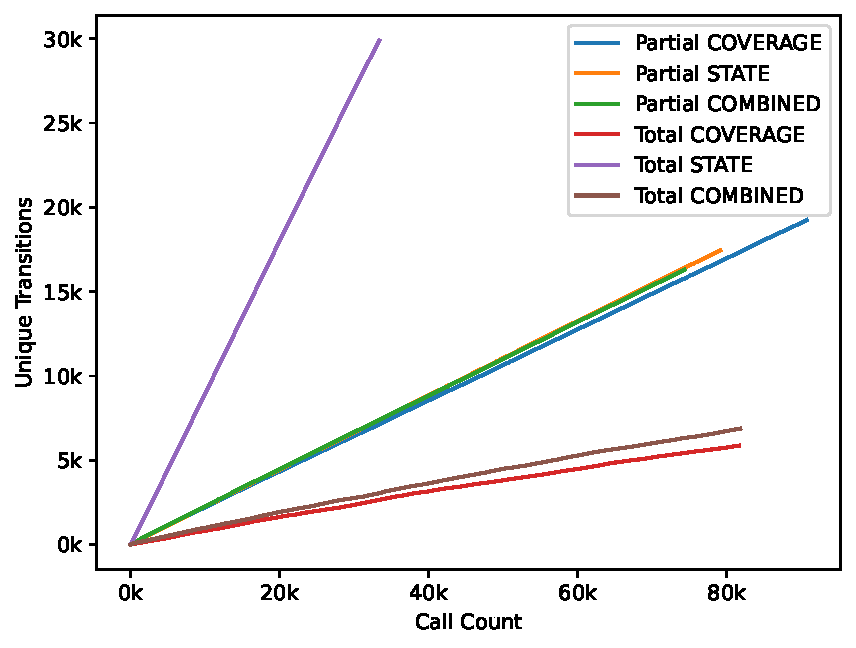
\includegraphics[width=0.48\textwidth]{charts/AlgoTether_ unique_transitions .pdf}
        \label{fig:AlgoTether_trans}
    }
    \hfill
    \subfloat[ExchangeToken][ExchangeToken]{
        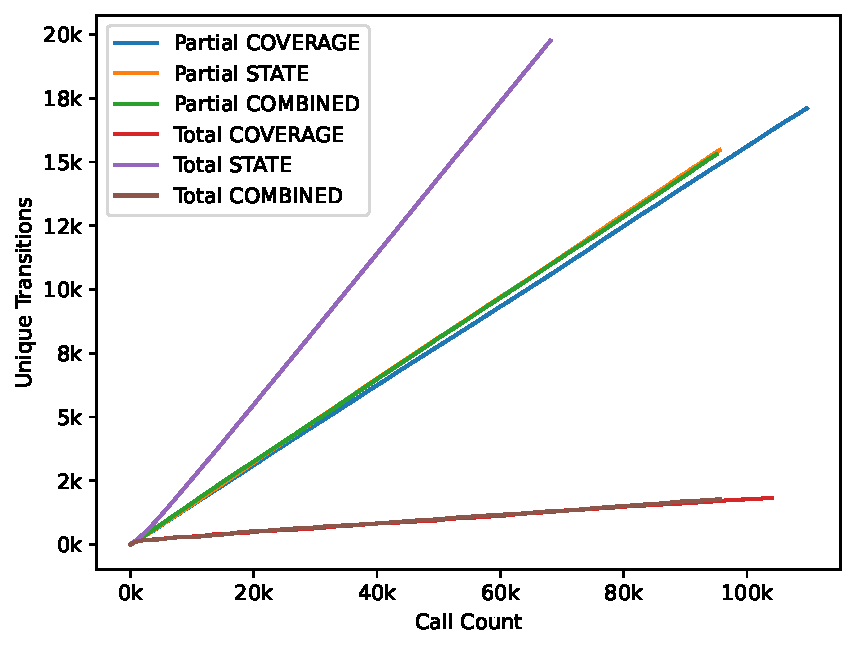
\includegraphics[width=0.48\textwidth]{charts/ExchangeToken_ unique_transitions .pdf}
        \label{fig:ExchangeToken_strans}
    }
    \caption{Average transitions achieved by AlgoTether and ExchangeToken for all configurations.}
    \label{fig:unique_transitions}
\end{figure}

\subsection*{State Discovery} \label{section:results-state-discovery}
For \textbf{RQ.2} we will look at the number of unique state transitions over the number of calls to the target contract.
Although a new state transition does not necessarily mean that a new state was discovered, it is a good approximation (since the maximal number of transitions is equal to number of states squared).
The best case scenario would be if the fuzzer discovers a new transition on every call.
In Figure \ref{fig:unique_transitions} we can see the unique transitions for the AlgoTether and ExchangeToken contracts.
Here we confirm our previous observations that we made for the Total State fuzzer in the case study in section \ref{section:case-study} which showed us that it is the most effective fuzzer at discovering new states.
These results also show that using the Total State fuzzer introduces an overhead since the number of calls is much lower even though the fuzzers run for the same amount of time.
The other configurations of the Total fuzzer in this metric are heavily underperforming by comparison to the Total State fuzzer and the Partial fuzzer. They are barely reaching around 5000 or 2000 transitions, while the other fuzzers reach between 15000 and 30000 transitions. The Total fuzzer with the Coverage or Combined driver also introduces more variance in the number of transitions, as can be seen in Figure \ref{fig:atrangetrans} and Figure \ref{fig:etrangetrans}.




To get a better understanding of the data we also calculated the ratio of transitions to calls for each configuration across all contracts.
We calculated the ratio for each contract by dividing the average number of transitions by the average number of calls for each configuration on the last call.
Best achievable ratio is 1.0 which would mean that the fuzzer discovered a new transition on every call.
For this data we created box plots shown in Figure \ref{fig:trans-ratio}.
The ratios are also shown for all contracts in Table \ref{table:trans-ratio}.
In the box plot it is shown that the Total State fuzzer has the highest median ratio, around 0.9, making it near perfect in terms of discovering new transitions.
The Partial fuzzers have a median of around 0.4 and the other Total fuzzers have a median of around 0.2.

\begin{figure}[hb]
    \centering
    \includegraphics*[width=0.8\textwidth]{charts/trans-ratio.pdf}
    \caption{Box plots for the ratio of transitions to calls for each fuzzer across all contracts.}\label{fig:trans-ratio}
\end{figure}

